\ifnpas
\subsection{Collision data samples}
\fi

\label{sec:dataSampleAndEventSelection}

The data sample was collected in 2011 at $\sqrt{s}=7$ TeV and corresponds to
an integrated luminosity of \intlumi.  Events are triggered by a single
\ifpas
calorimeter jet.
\else
{\tt CaloJet}.
\fi
As the instantaneous luminosity increased with time,
different thresholds are used in different time periods.
We use the same trigger strategy as the standard dijet
analysis in Ref.~\cite{CMS-PAS-QCD-11-004}. 
Offline, one jet (reconstructed by the particle flow algorithm) is required to satisfy $\pt > 30$~\GeVc.
The efficiencies of 
these triggers are shown in Figure~\ref{figs:efficiency_HLT}. 


\ifnpas
\begin{table}
\begin{center}
\begin{tabular}{ |l|c| }
\hline
Dataset                                 &       Luminosity ($pb^{-1}$) \\
\hline
/Jet/Run2011A-May10ReReco/AOD             &       189                   \\
/Jet/Run2011A-PromptReco-v$*$/AOD         &       1849                   \\
/Jet/Run2011B-PromptReco-v$*$/AOD         &       2523                   \\
\hline
\end{tabular} 
\end{center}
\caption{Summary of 7 \TeV collision data used in this analysis. The certification
used for these data is {\tt Cert\_160404-180252\_7TeV\_PromptReco\_Collisions11\_JSON.txt}.}
\label{table:dataset}
\end{table}


\begin{table}
\begin{center}
\begin{tabular}{|l|r|r|r|}
\hline
Process                      & Cross section (pb)   & Generator & Number \\
\hline
\tt{QCD\_Pt-15to3000\_TuneZ2\_Flat\_7TeV\_pythia6}  & 2.21e10 & \PYTHIA & 10960800\\
\tt{QCD\_Pt-15to3000\_Tune4C\_Flat\_7TeV\_pythia8}  & 2.51e10 & \PYTHIAEIGHT & 1060650 \\
\tt{QCD\_Pt-15to3000\_Tune23\_Flat\_7TeV\_herwigpp} & 2.31e10 & \HERWIG & 10430351 \\
\hline
\end{tabular}
\end{center}
\caption{Summary of the simulated Monte Carlo samples used in this analysis. All samples use the
``Scenario 3'' \tt{Summer11-PU\_S3\_START42\_V11-v2} pileup scenario.}
\label{table:mcdataset}
\end{table}


\begin{figure}[htb]
\centering
\begin{tabular}{|l|r|r|}
\hline
Trigger & Effective lumi (\invpb) & Effective prescale\\
\hline
\verb!HLT_Jet60!  & 0.407  & 12300.0 \\
\verb!HLT_Jet110! & 7.27   & 690.0   \\
\verb!HLT_Jet190! & 152.6  & 32.9    \\ 
\verb!HLT_Jet240! & 521.5  & 9.6     \\
\verb!HLT_Jet370! & 4067.0 & 1.0     \\
\hline
\end{tabular}
  \caption[Jet triggers]{Jet triggers used, plus effective luminosity and precale.}
  \label{fig:trigger}
\end{figure}
\fi


The parton distribution functions used were from {\rm CTEQ 6l}~\cite{cteq}.

{\bf TODO!:}Variations were checked for the uncertainties according to
Ref.~\cite{pdf4lhc} and found to be negligible. 

Events were fully simulated
and reconstructed via the CMS
simulation and reconstruction software. 

\subsection{Reconstruction and event preselection}

\ifnpas
All data are reconstructed using CMSSW 4.2.x.
\fi
\label{sec:preselection}
\label{sec:reconstruction}
Event data are reconstructed using the particle-flow reconstruction algorithm~\cite{particleflow},
which attempts to reconstruct all stable particles in an event by combining information from
all subdetectors. The algorithm categorizes all particles into five types: muons,
electrons, photons, charged and neutral hadrons. The resulting particle flow candidates are passed
to each jet clustering algorithm described in Sec.~\ref{sec:algos} to create "particle flow jets", 
as implemented in FastJet version 2.4.2 \cite{fastjet1,fastjet2}.



%An extra correction is applied to the data to account for a residual
%nonlinearity that is not observed in the simulation. No pileup
%corrections are applied. 
Charged hadrons identified as pileup are removed from the inputs to the jet clustering algorithms.
The charged hadrons are classified as belonging to a 
pileup vertex when they are used to reconstruct a vertex that is not the highest $\pt$ primary vertex. 
Furthermore, charged leptons with an isolation
of 15\% (muons) or 20\% (electrons) of the lepton transverse momentum 
are also removed, where the isolation is defined as the
fraction of energy from charged particles, neutral particles, and photons (counted separately). 

% After these subtractions, aside from the true constituents of the jets,
% this leaves only the neutral component of pileup,
% This is removed by applying a residual

After these subtractions, only the neutral component of pileup remains;
it is removed by applying a residual area-based correction as described in
Ref.~\cite{jetarea_fastjet,jetarea_fastjet_pu}. 
The mean $\pt$ per unit area
is computed with the $k_{\mathrm T}$ algorithm with the ``active area'' method,
with a distance parameter of 0.6, and the
jet energy is corrected by the amount of pileup expected in the jet
area. The ``active area'' method adds a large number of infinitely
soft ``ghost'' particles to the clustering sequence to examine which
jet they are clustered into, and the area is computed by the set of
points for each jet. The active area method is also used to compute
the jet area for the jets in the analysis. 
$\eta$-dependent jet corrections are also necessary,
due to the different responses in the endcap
and barrel calorimeters. The amount of energy expected from underlying
event is added back into the jet. 


The pileup-subtracted jet four momenta are finally 
corrected for nonlinearities in $\eta$ and $\pt$
with simulated data, with a residual $\eta$-dependent correction added 
to correct for the difference in simulated and true responses~\cite{jec_spring10}.  Constituents
of the jet (i.e. subjets) are not corrected, and algorithmic procedures are done on uncorrected jet
energies. 
The jet corrections used are specifically derived for the AK7 jet algorithm.


% These corrections are then
% applied as 
% \begin{equation}
% \pt^{PU-corr} = \pt^{RAW} \times \left( 1 - F(\eta) \times \frac{A_{jet} (\rho - <\rho_{UE}>)}{<A_{jet}> <(\rho_{PU,NPV=1})>} \right)
% \end{equation}
% The function $F(\eta)$ is an $\eta$-dependent correction designed to correct for
% different responses between the barrel and endcap calorimeters.
% It is derived from an assumption of a linear dependence of jet
% momenta as a function of the number of reconstructed primary vertices, 
% and then computed over a range of jet pseudorapidities. 
% The area of the jet $A_{jet}$ is computed as described in Ref~\cite{fastjet_area},
% and depends ont he jet algorithm. The mean $\pt$ per unit area for underlying
% event ($\rho_{UE}$) is added back into the jet, since the cachement area approach
% subtracts this as well (which should, however, be added in the jet momentum measurement
% to be consistent with theoretical predictions). The average jet area $<A_{jet}>$ is
% derived for the algorithm in question in a dijet sample, and $<\rho_{PU,NPV=1}>$ is the
% expected average mean $\pt$ per unit area in events with exactly one primary vertex. 



The following preselection is applied.
\ifnpas
\begin{itemize}

\item The event must have a good primary vertex as computed by a deterministic annealing filter (DAF)
($\vert z_\text{Primary Vertex}\vert < 24$ cm, $N_\text{DOF} > 6$).
\item Events are required to have at least two jets with
        \begin{itemize}
          \item $\pt > 50 \GeVc$, $|y| < 2.5$
        \item Loose particle flow jet identification~\cite{jetid} is applied
        \end{itemize}
\item Beam background events are removed using the following requirements:
        \begin{itemize}
        \item In events with at least 10 tracks, a minimum of 25\% of
          these tracks must be high purity tracks.
        \end{itemize}
\end{itemize}
\else
The events must have a good primary vertex as computed by a
deterministic annealing filter (DAF). Furthermore, beam backgrounds
are removed by requiring that events with at least 10 tracks 
have at least 25\% of the tracks satisfying high purity tracking
requirements.
Events are required to have at least two AK7 jets with
$\pt > 50$ \GeVc and $|y| < 2.5$
and each jet must satisfy jet quality criteria \cite{particleflow}. 
\fi


\ifnpas
This measurement depends on the jet mass resolution and response,
especially in the assignment of bin size for the measurement. 
The reconstructed jet mass divided by the generated jet mass
versus generated jet mass was investigated in \PYTHIA MC. To estimate
the response and resolution, a Gaussian was fitted to the $m_{j}^{GEN}$
slices, and the response corresponds to the mean, while the resolution
corresponds to the width of the fits. 

Figure~\ref{figs:response_histAK7MjetResponseVsPtAvg}
shows the response for ungroomed, filtered, trimmed, and pruned jets
versus $m_{J}^{GEN}$ for various $\pt$ bins, and 
Figure~\ref{figs:resolution_histAK7MjetResponseVsPtAvg}
shows the resolution. For some specific numbers, the jet mass resolution is
around 5-10 \GeVcc for $m_{J}^{GEN} = 50$ \GeVcc, and around 10 \GeVcc
for $m_{J}^{GEN} = 200$ \GeVcc. The chosen bin size of 10 \GeVcc is 
well-motivated here. 
\fi


\begin{figure}[htbp]
\centering
\subfigure{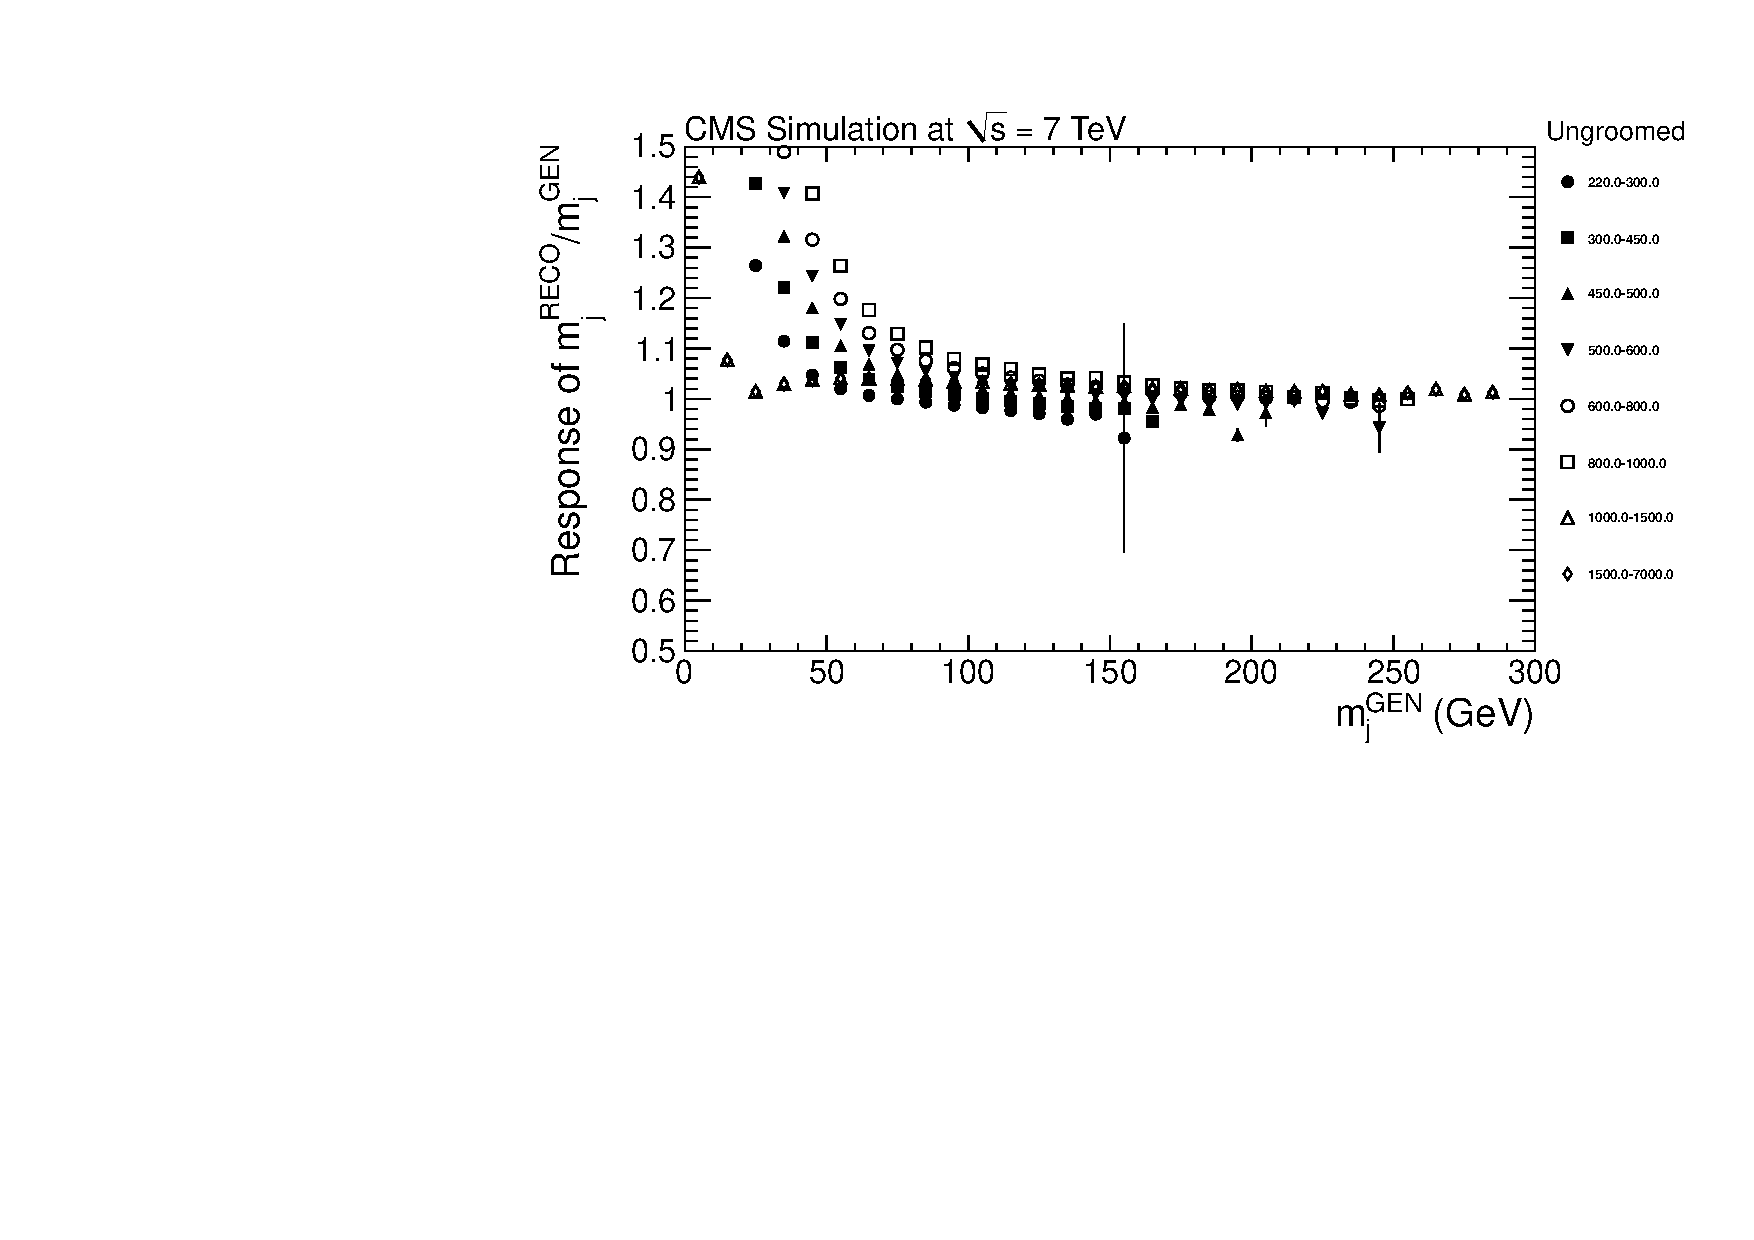
\includegraphics[width=0.5\textwidth]{figs/response_histAK7MjetResponseVsPtAvg}}
\subfigure{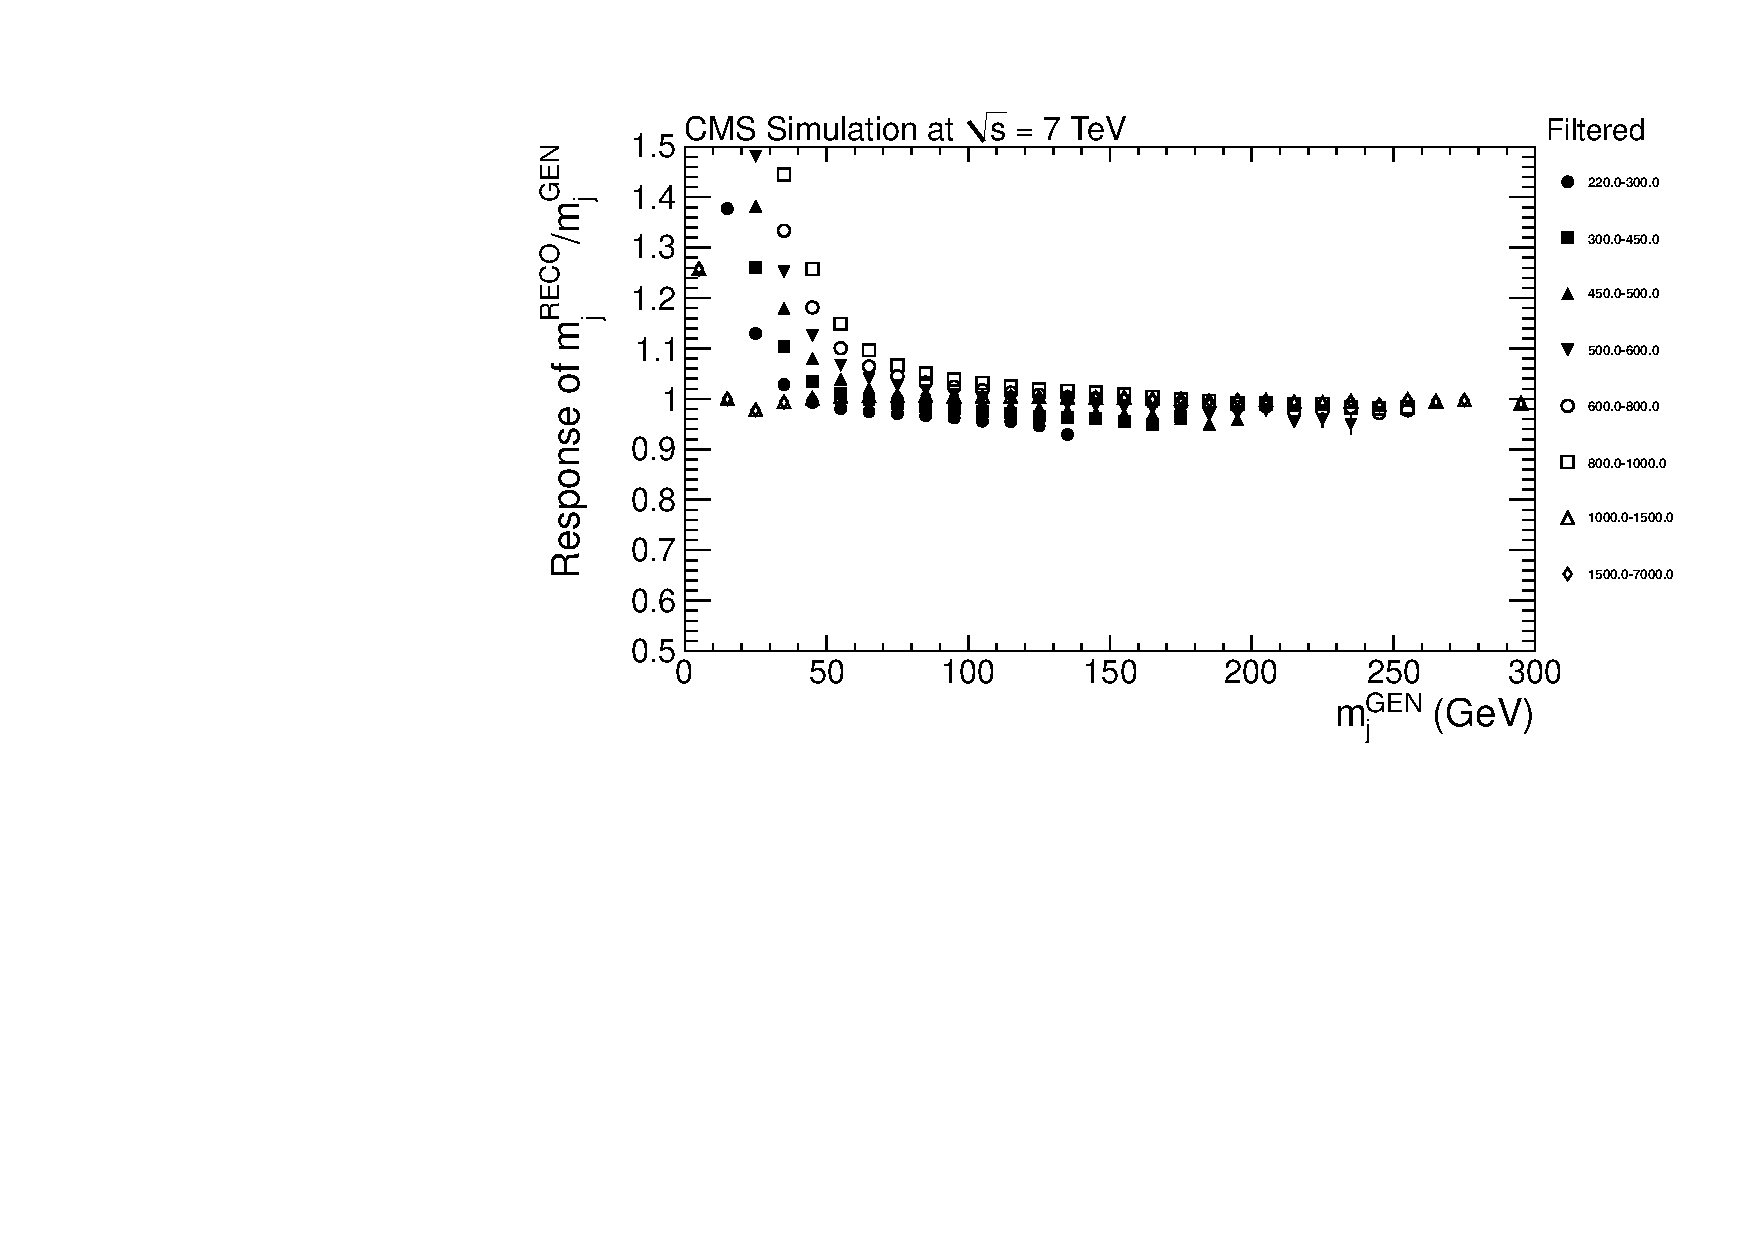
\includegraphics[width=0.5\textwidth]{figs/response_histAK7MjetResponseVsPtAvg_Filtered}}\\
\subfigure{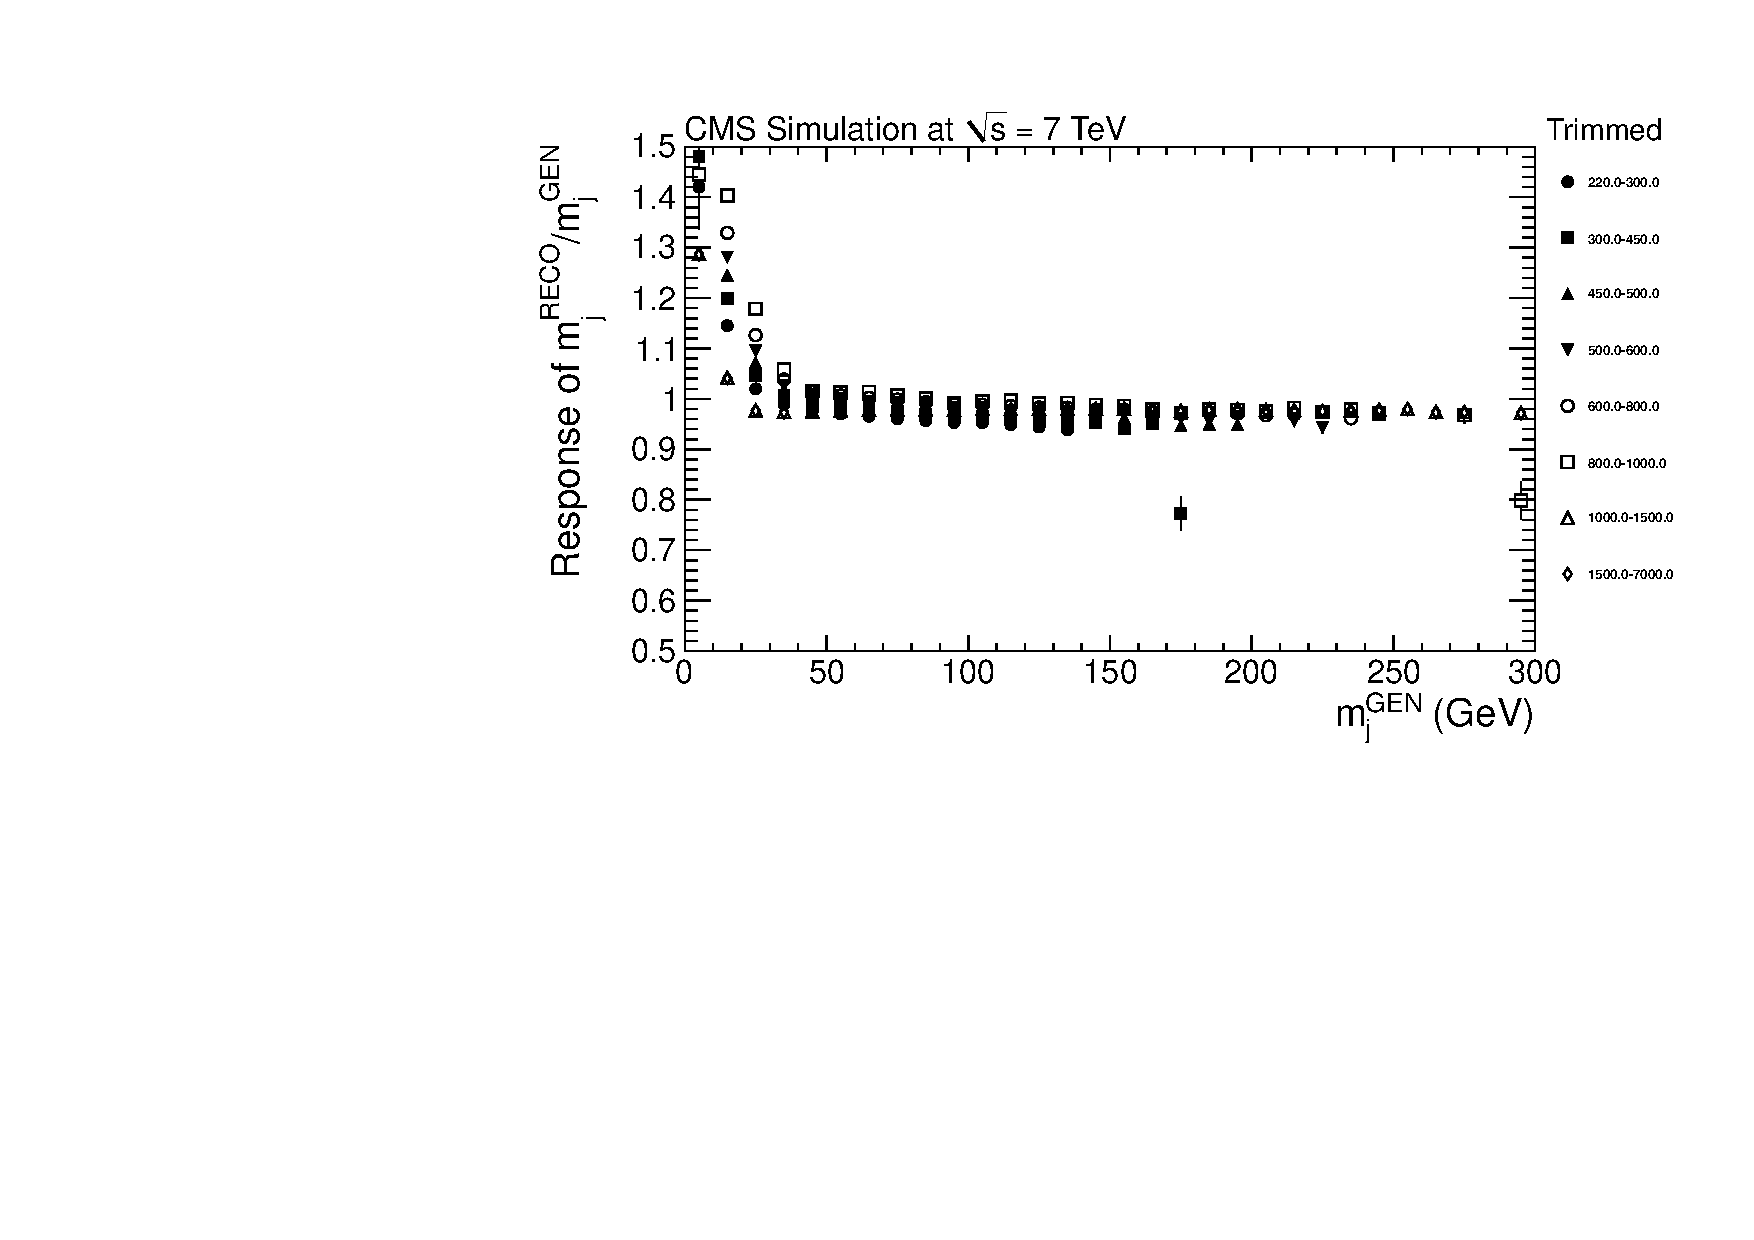
\includegraphics[width=0.5\textwidth]{figs/response_histAK7MjetResponseVsPtAvg_Trimmed}}
\subfigure{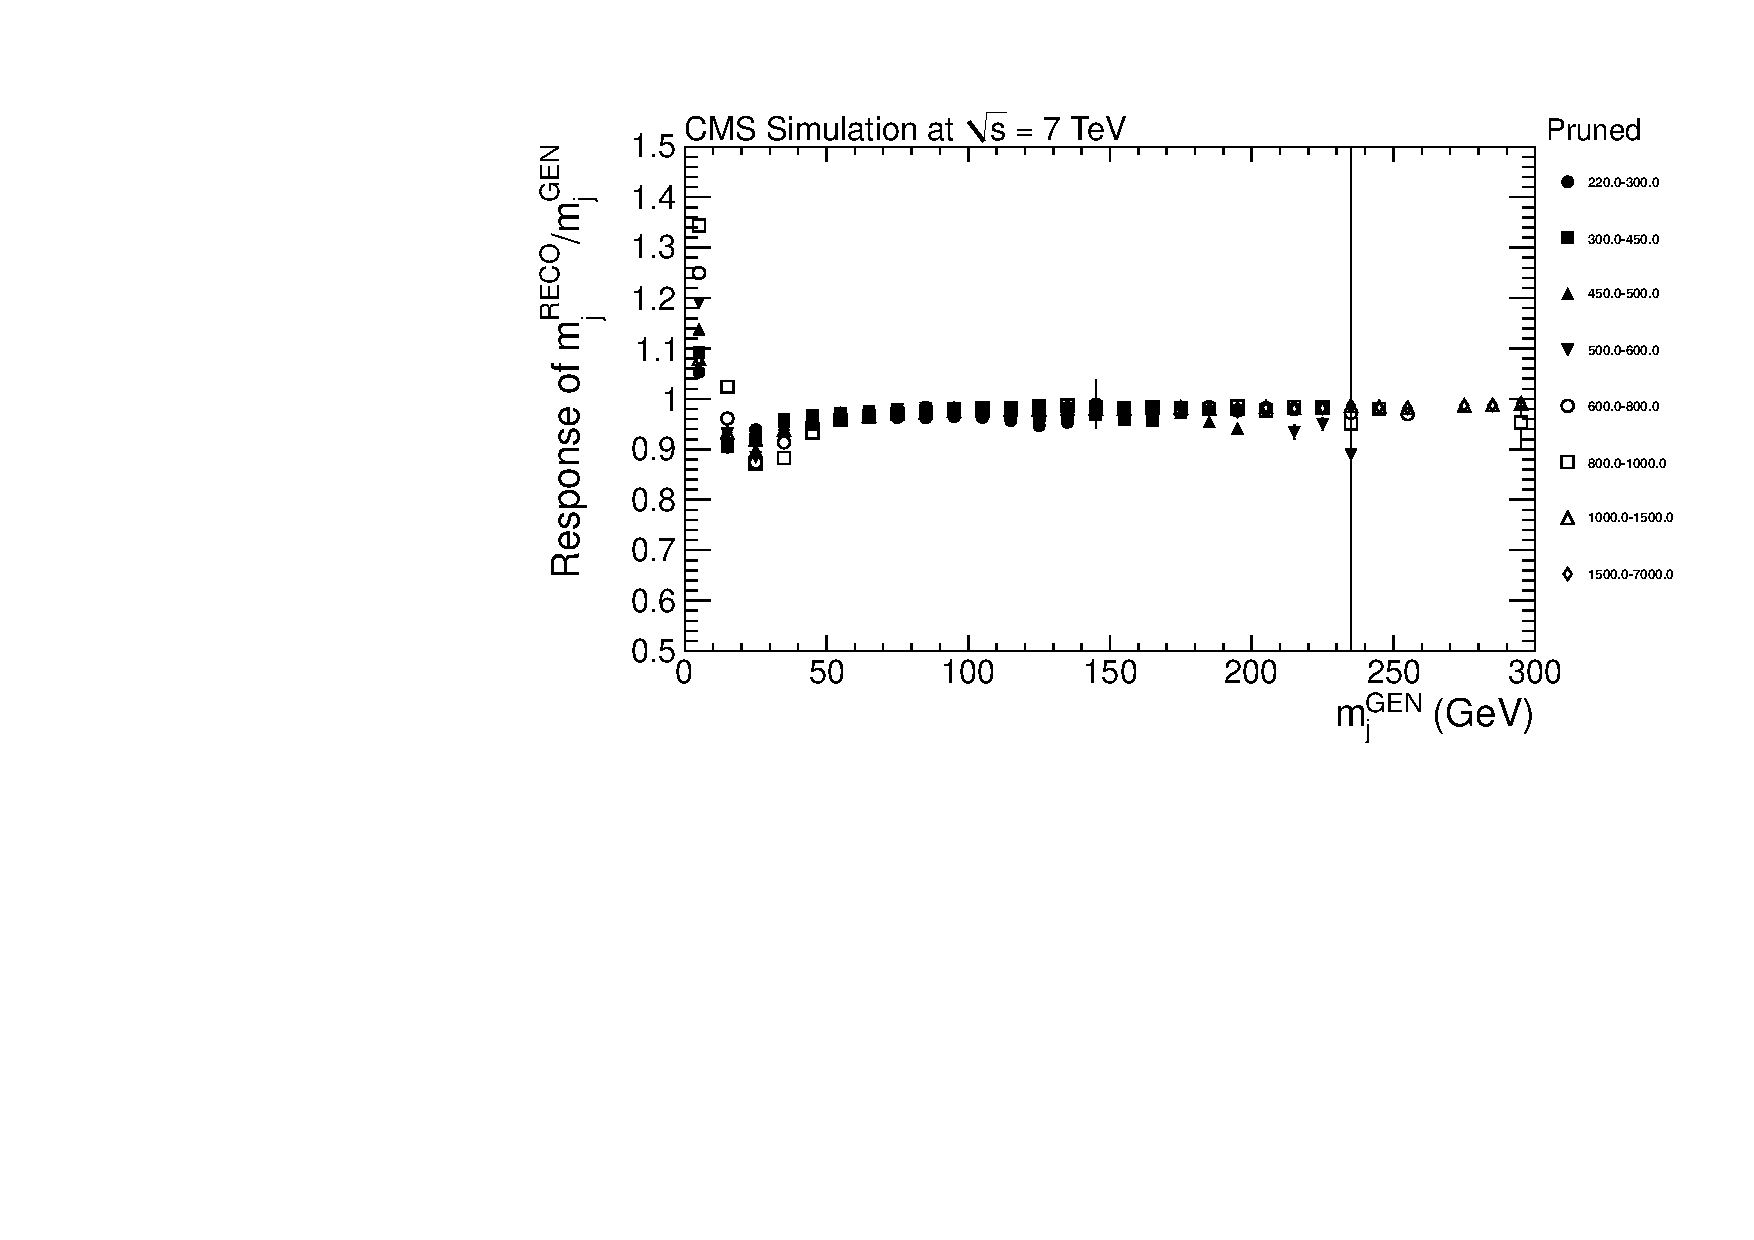
\includegraphics[width=0.5\textwidth]{figs/response_histAK7MjetResponseVsPtAvg_Pruned}}
\caption{Mean of $m_{J}^{RECO} / m_{J}^{GEN}$ in slices of 
$m_{J}^{GEN}$, for various $\pt$ bins, for each of the grooming
algorithms. This corresponds to the jet response. 
\label{figs:response_histAK7MjetResponseVsPtAvg}}
\end{figure}


\begin{figure}[htbp]
\centering
\subfigure{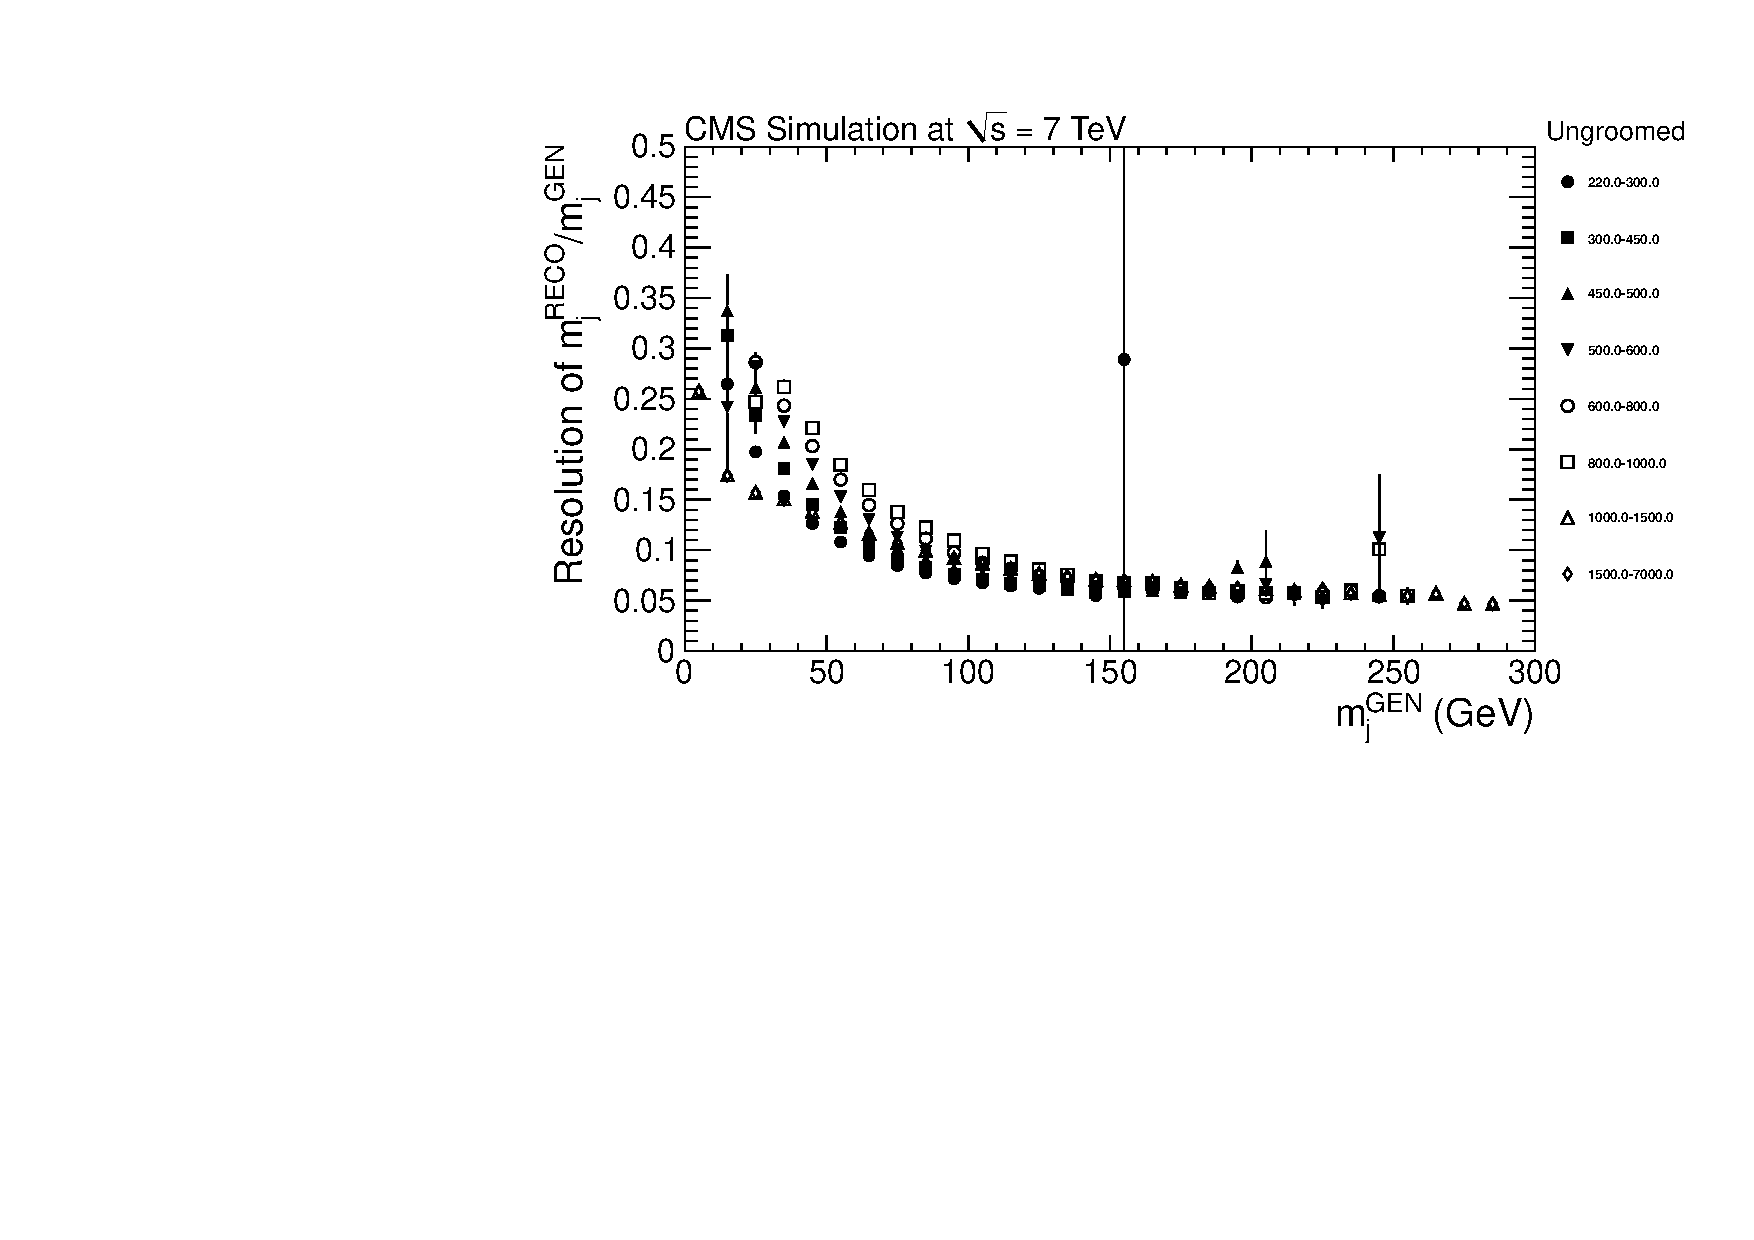
\includegraphics[width=0.5\textwidth]{figs/resolution_histAK7MjetResponseVsPtAvg}}
\subfigure{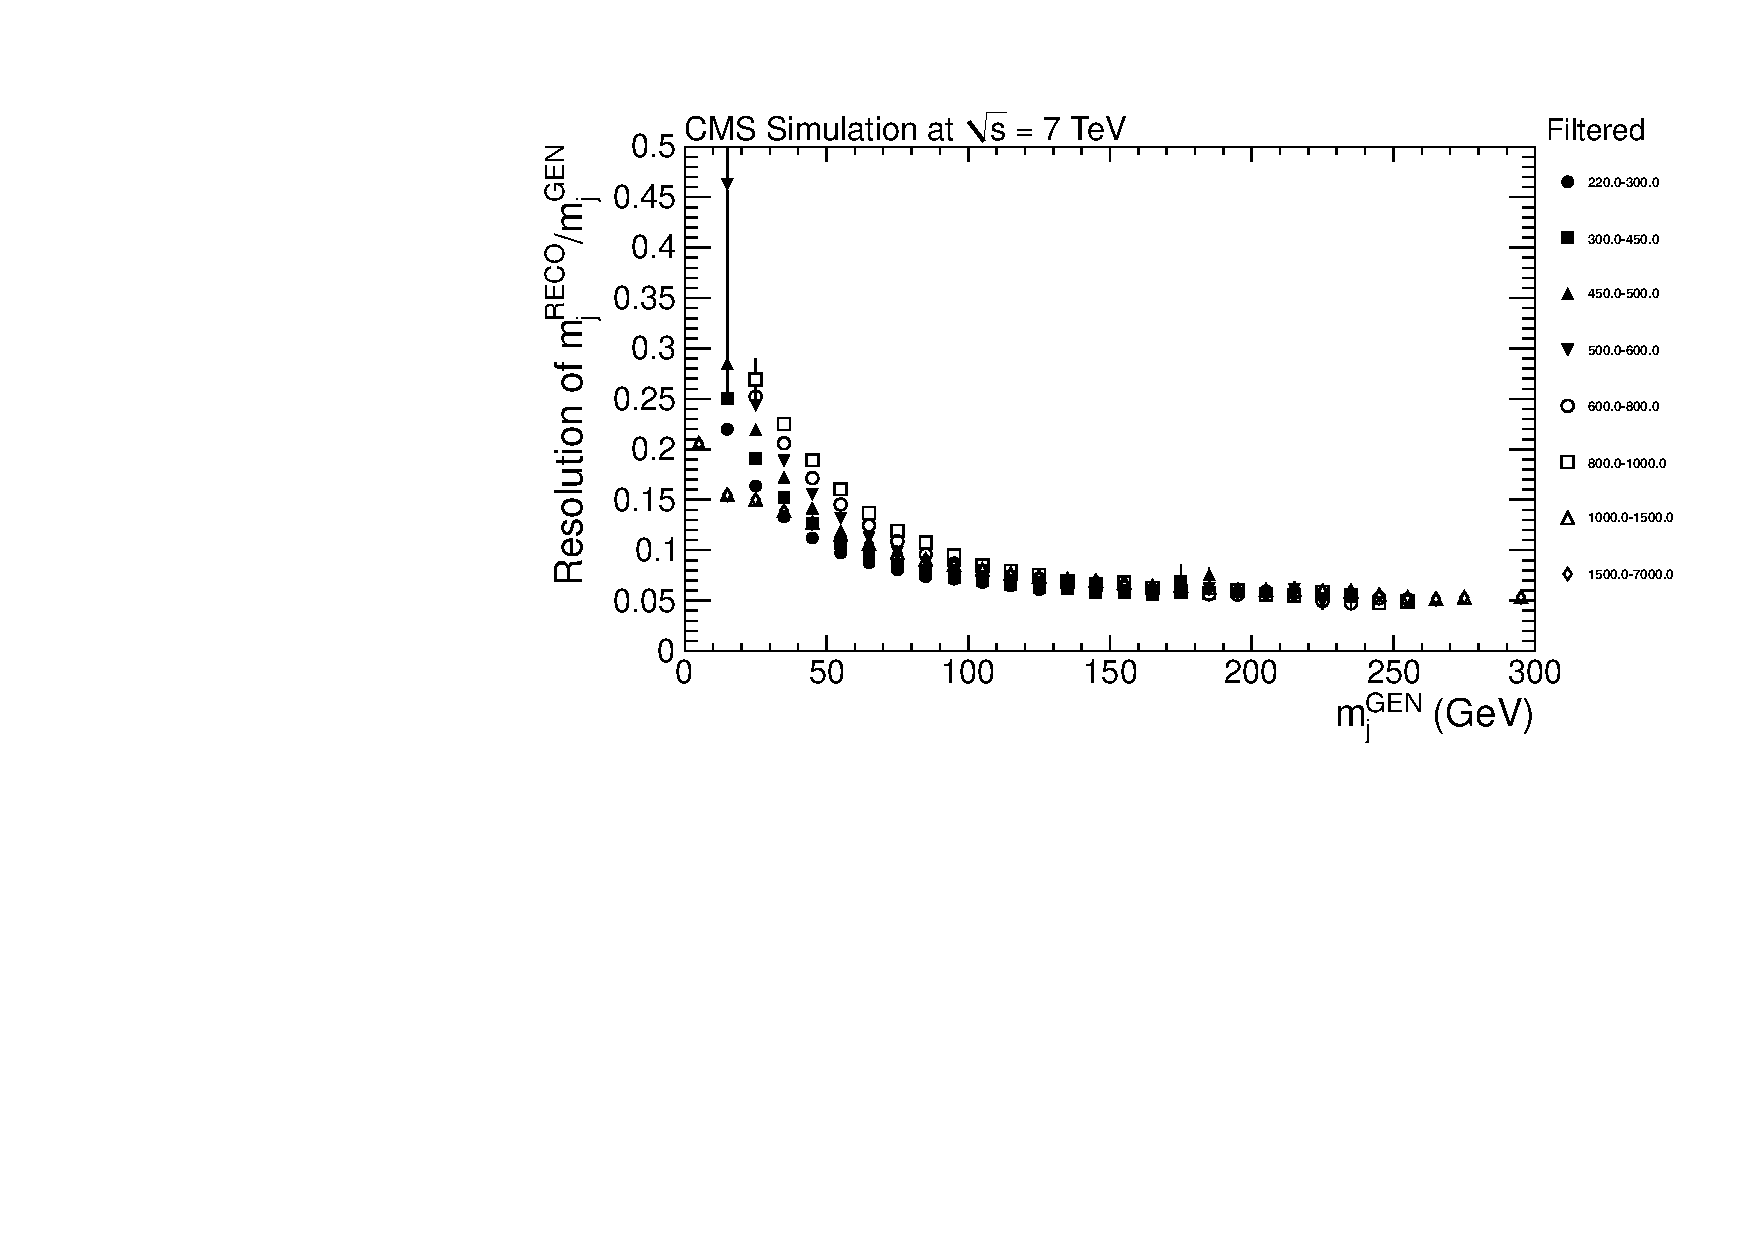
\includegraphics[width=0.5\textwidth]{figs/resolution_histAK7MjetResponseVsPtAvg_Filtered}}\\
\subfigure{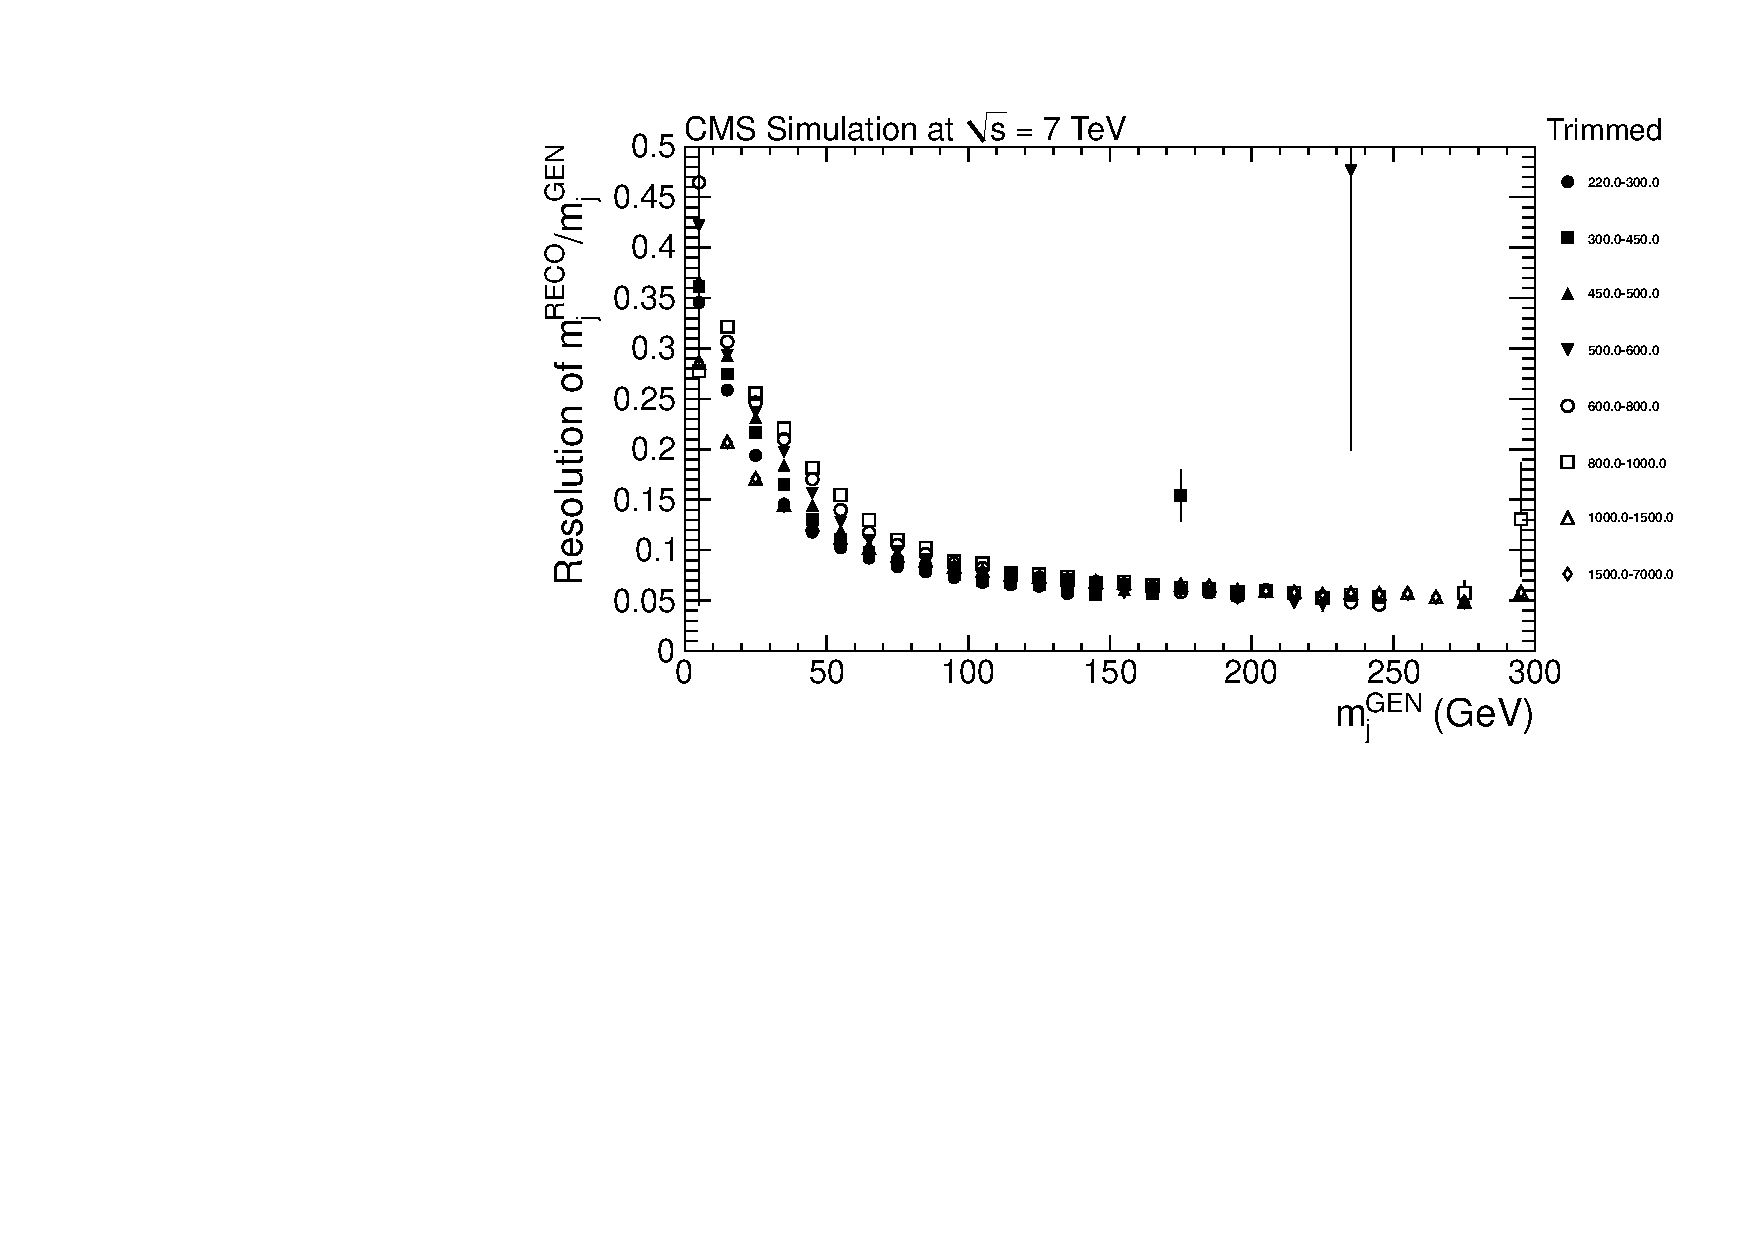
\includegraphics[width=0.5\textwidth]{figs/resolution_histAK7MjetResponseVsPtAvg_Trimmed}}
\subfigure{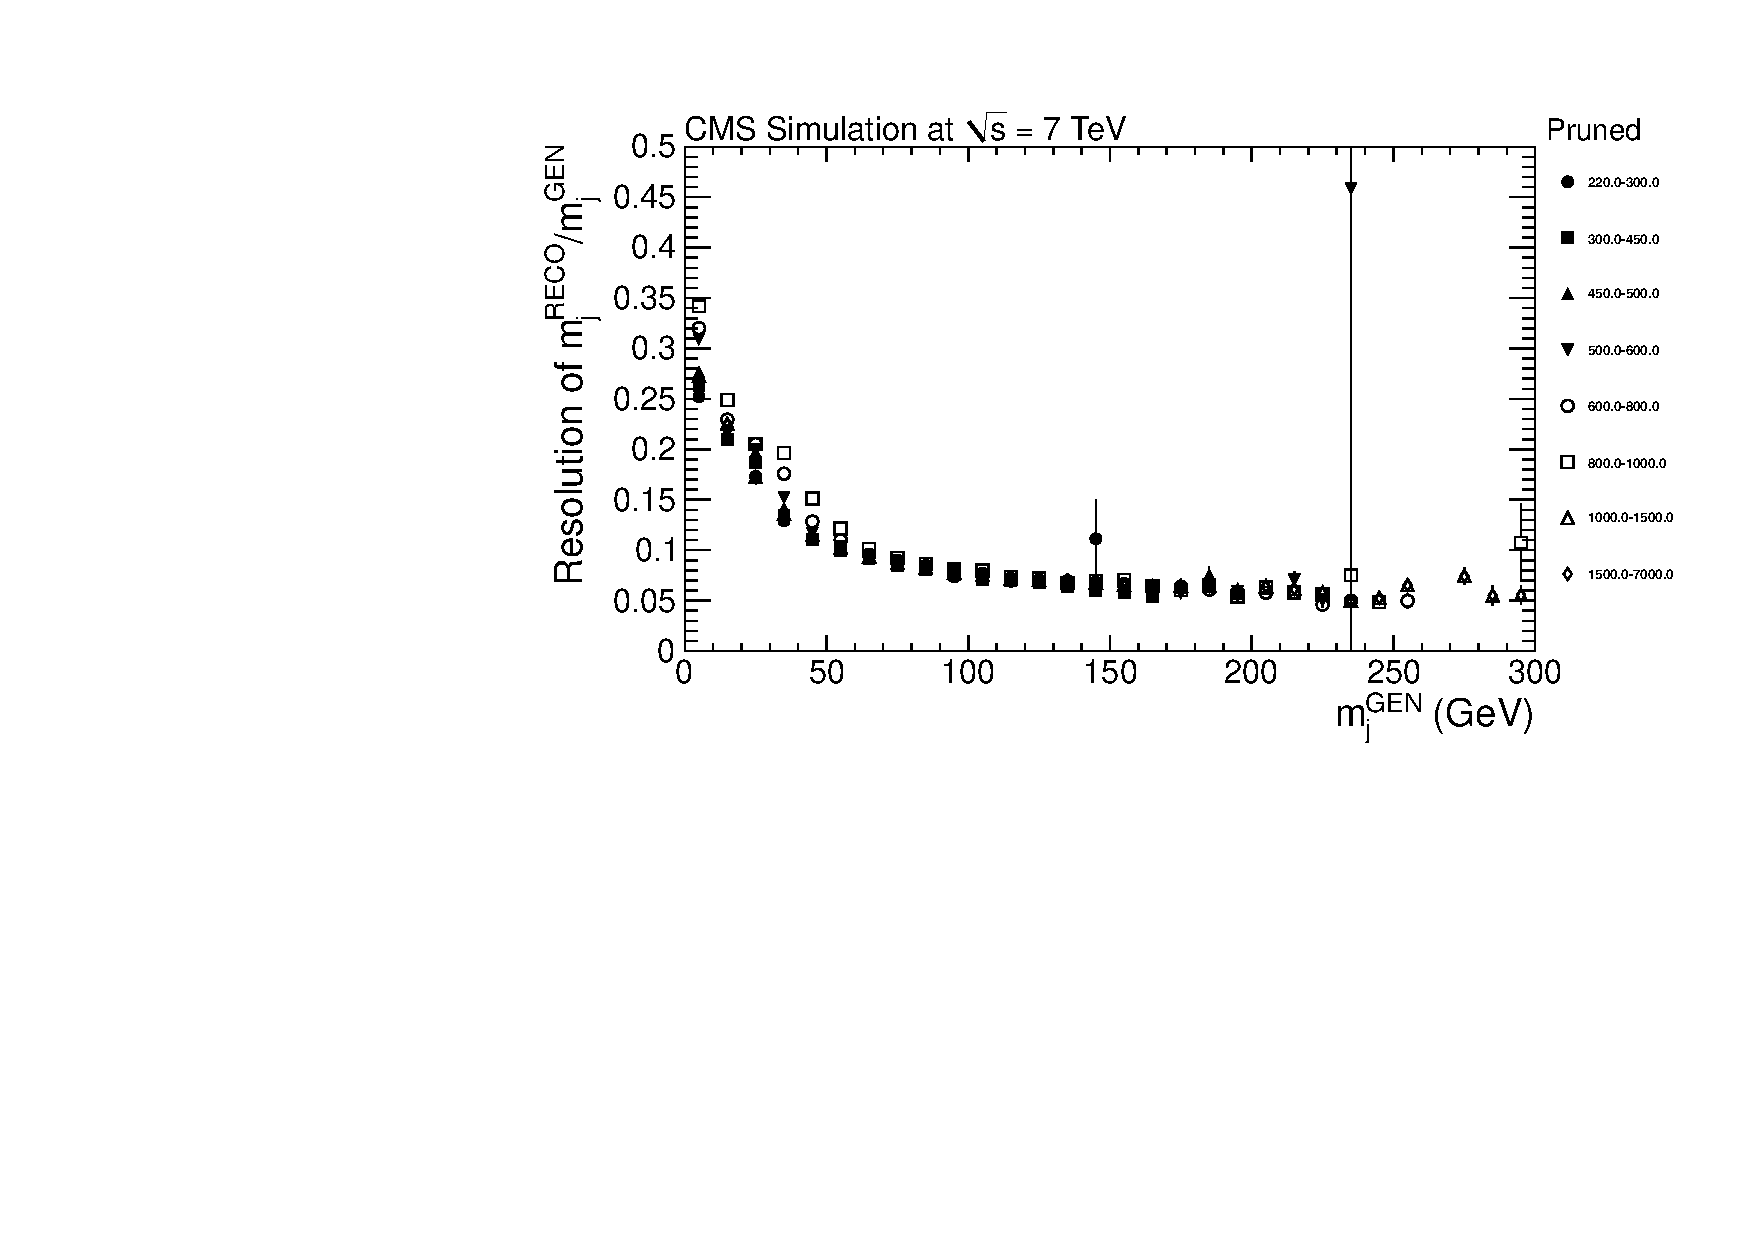
\includegraphics[width=0.5\textwidth]{figs/resolution_histAK7MjetResponseVsPtAvg_Pruned}}
\caption{Width of $m_{J}^{RECO} / m_{J}^{GEN}$ in slices of 
$m_{J}^{GEN}$, for various $\pt$ bins, for each of the grooming
algorithms. This corresponds to the jet resolution. 
\label{figs:resolution_histAK7MjetResponseVsPtAvg}}
\end{figure}


\subsection{Trigger assignment}
\label{sec:trigAssignment}

The triggers that were used in this analysis have partially overlapping phase space. 
The lower-threshold triggers have high prescales in order to accommodate higher
trigger rates, and the $\pt$ selections on these triggers are only one-sided,
hence lower-threshold triggers have overlapping phase space with higher-threshold
triggers. To correctly assign events to a specific trigger, the
strategy used is to compute the trigger efficiency as a function
of $\pt^{AVG}$ and select a region in the trigger plateau, then
assign one trigger per $\pt^{AVG}$ region. Table~\ref{TriggerTurnOns}
shows the trigger threshold for each trigger.
Figure~\ref{figs:efficiency_HLT}
shows the efficiency turn-ons computed with respect to the
next lowest trigger. The efficiency is defined as:

\begin{equation}
\epsilon = \frac{L_{A-1} N_{A}}{L_{A} N_{A-1}}
\end{equation}

where $\epsilon$ is the efficiency, $N_{A}$ is the number of
events that pass trigger with threshold $A$, and $L_{A}$ is the
effective luminosity of the trigger with threshold $A$ as shown
in Tab.~\ref{fig:trigger}. 


In the case of using
groomed jets, the trigger assignment is still used from the ungroomed
collection, and hence the trigger assignment is identical for all
algorithms, whether or not they are groomed. 
The trigger binning is selected such that the efficiency is in the
plateau. 

\begin{figure}[htbp]
\centering
\subfigure{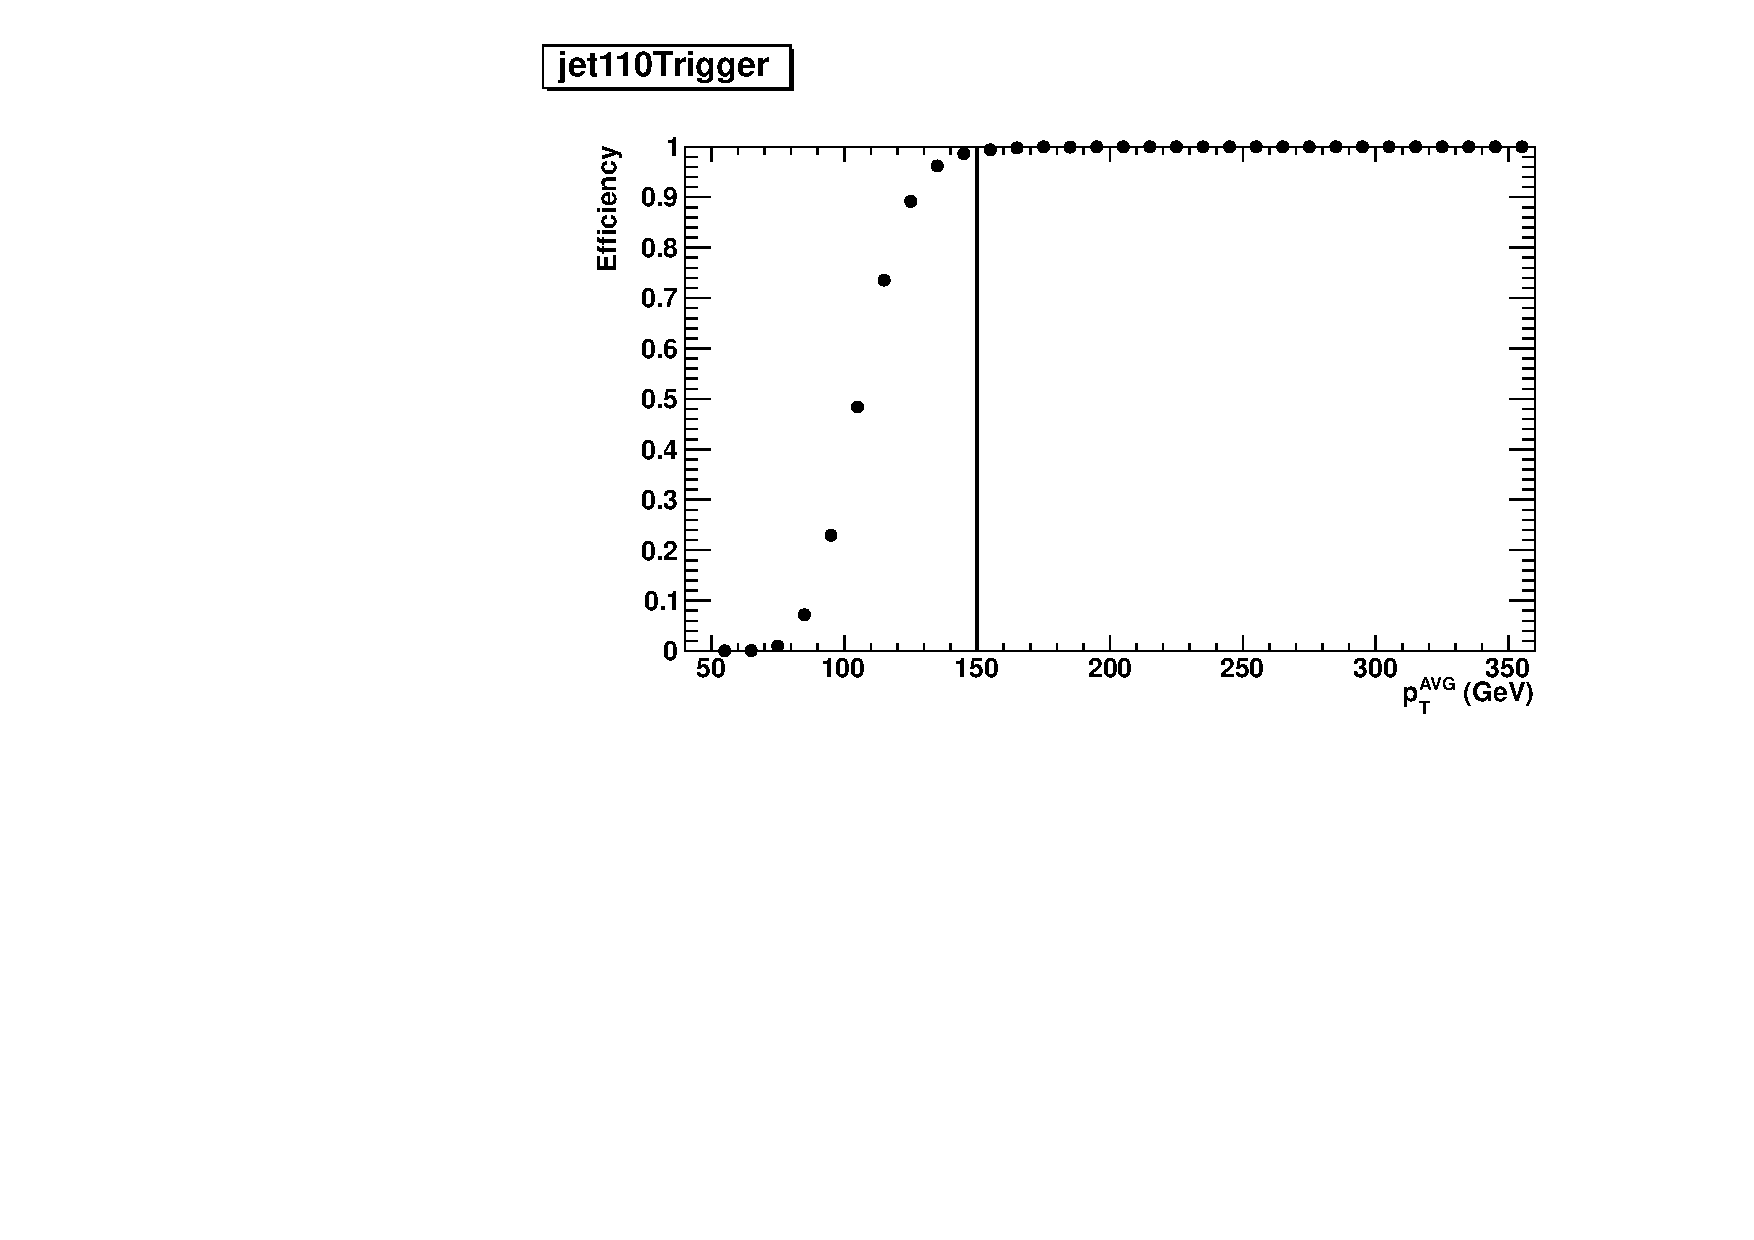
\includegraphics[width=0.6\textwidth]{figs/efficiency_jet110Trigger}}
\subfigure{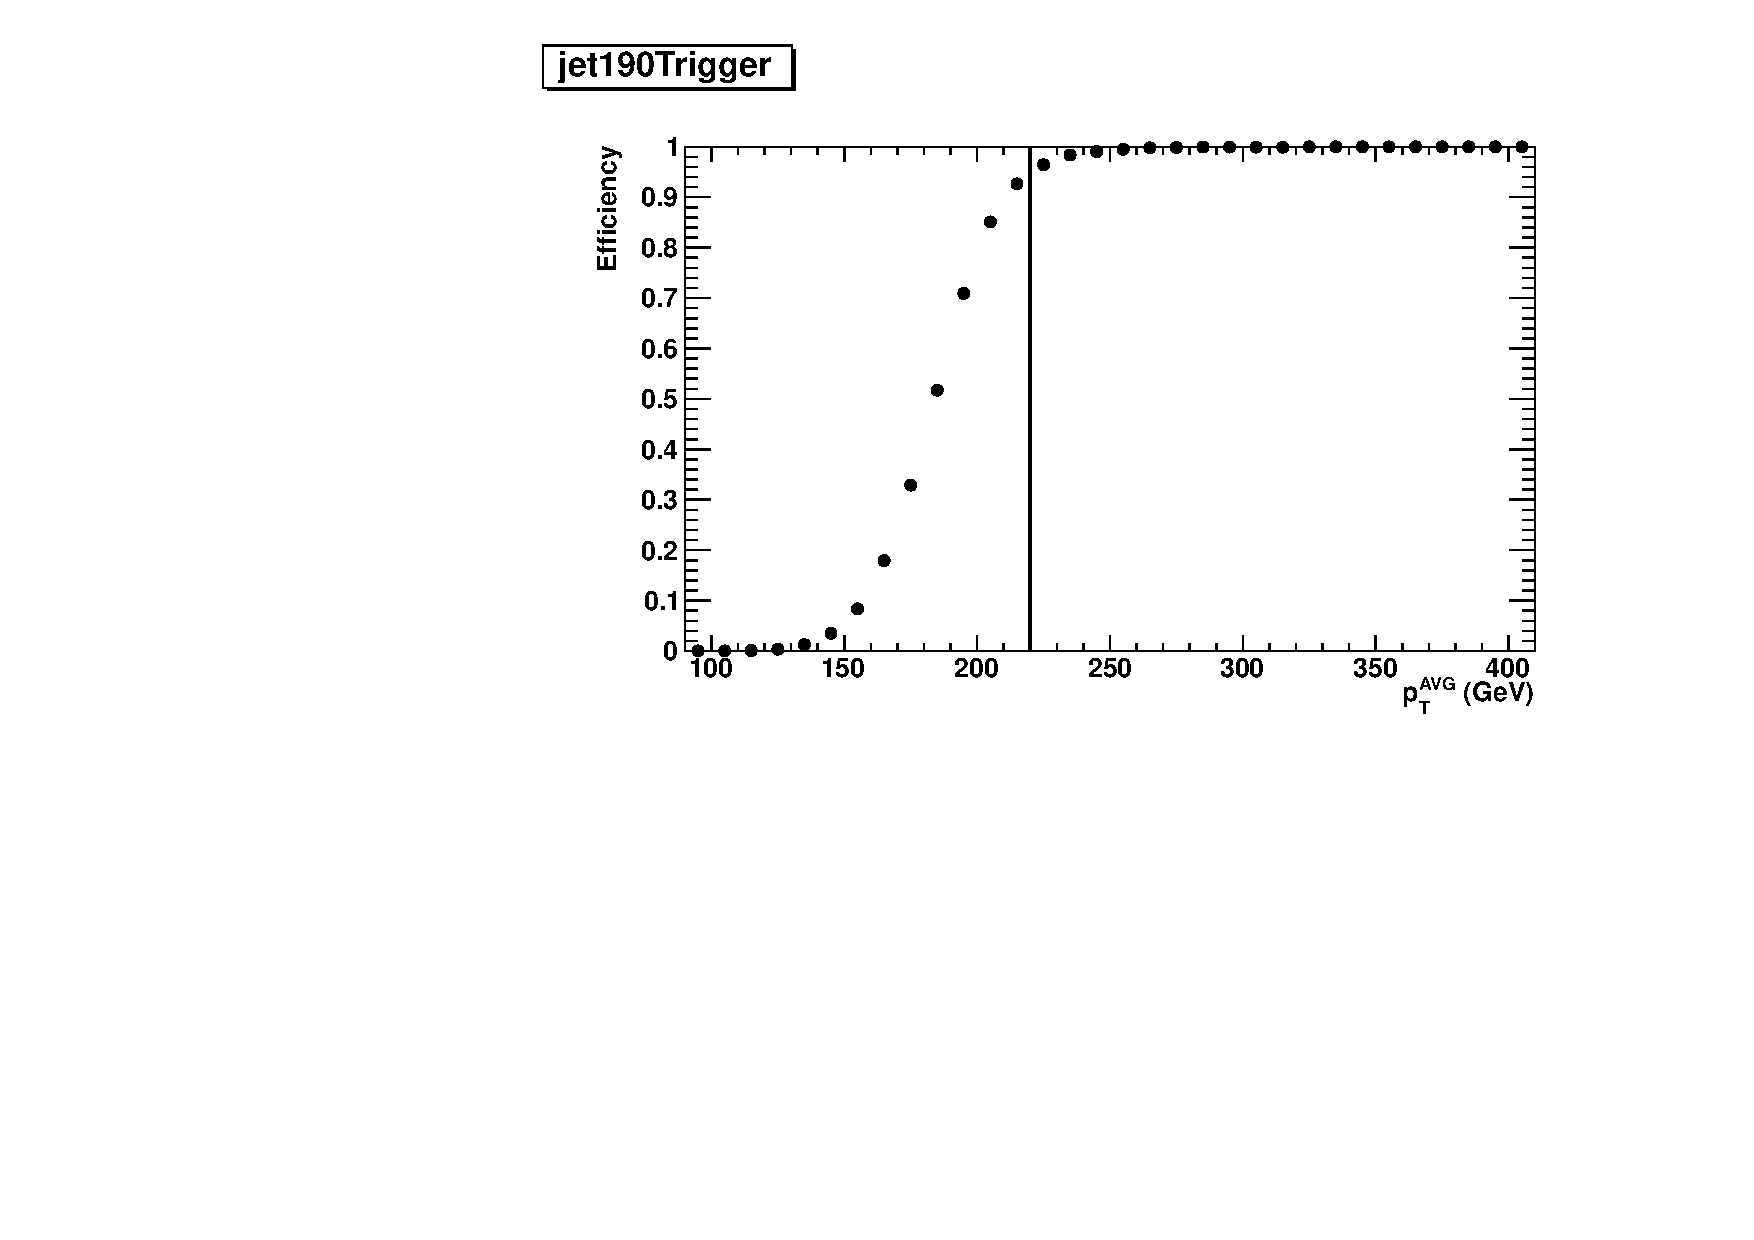
\includegraphics[width=0.6\textwidth]{figs/efficiency_jet190Trigger}}\\
\subfigure{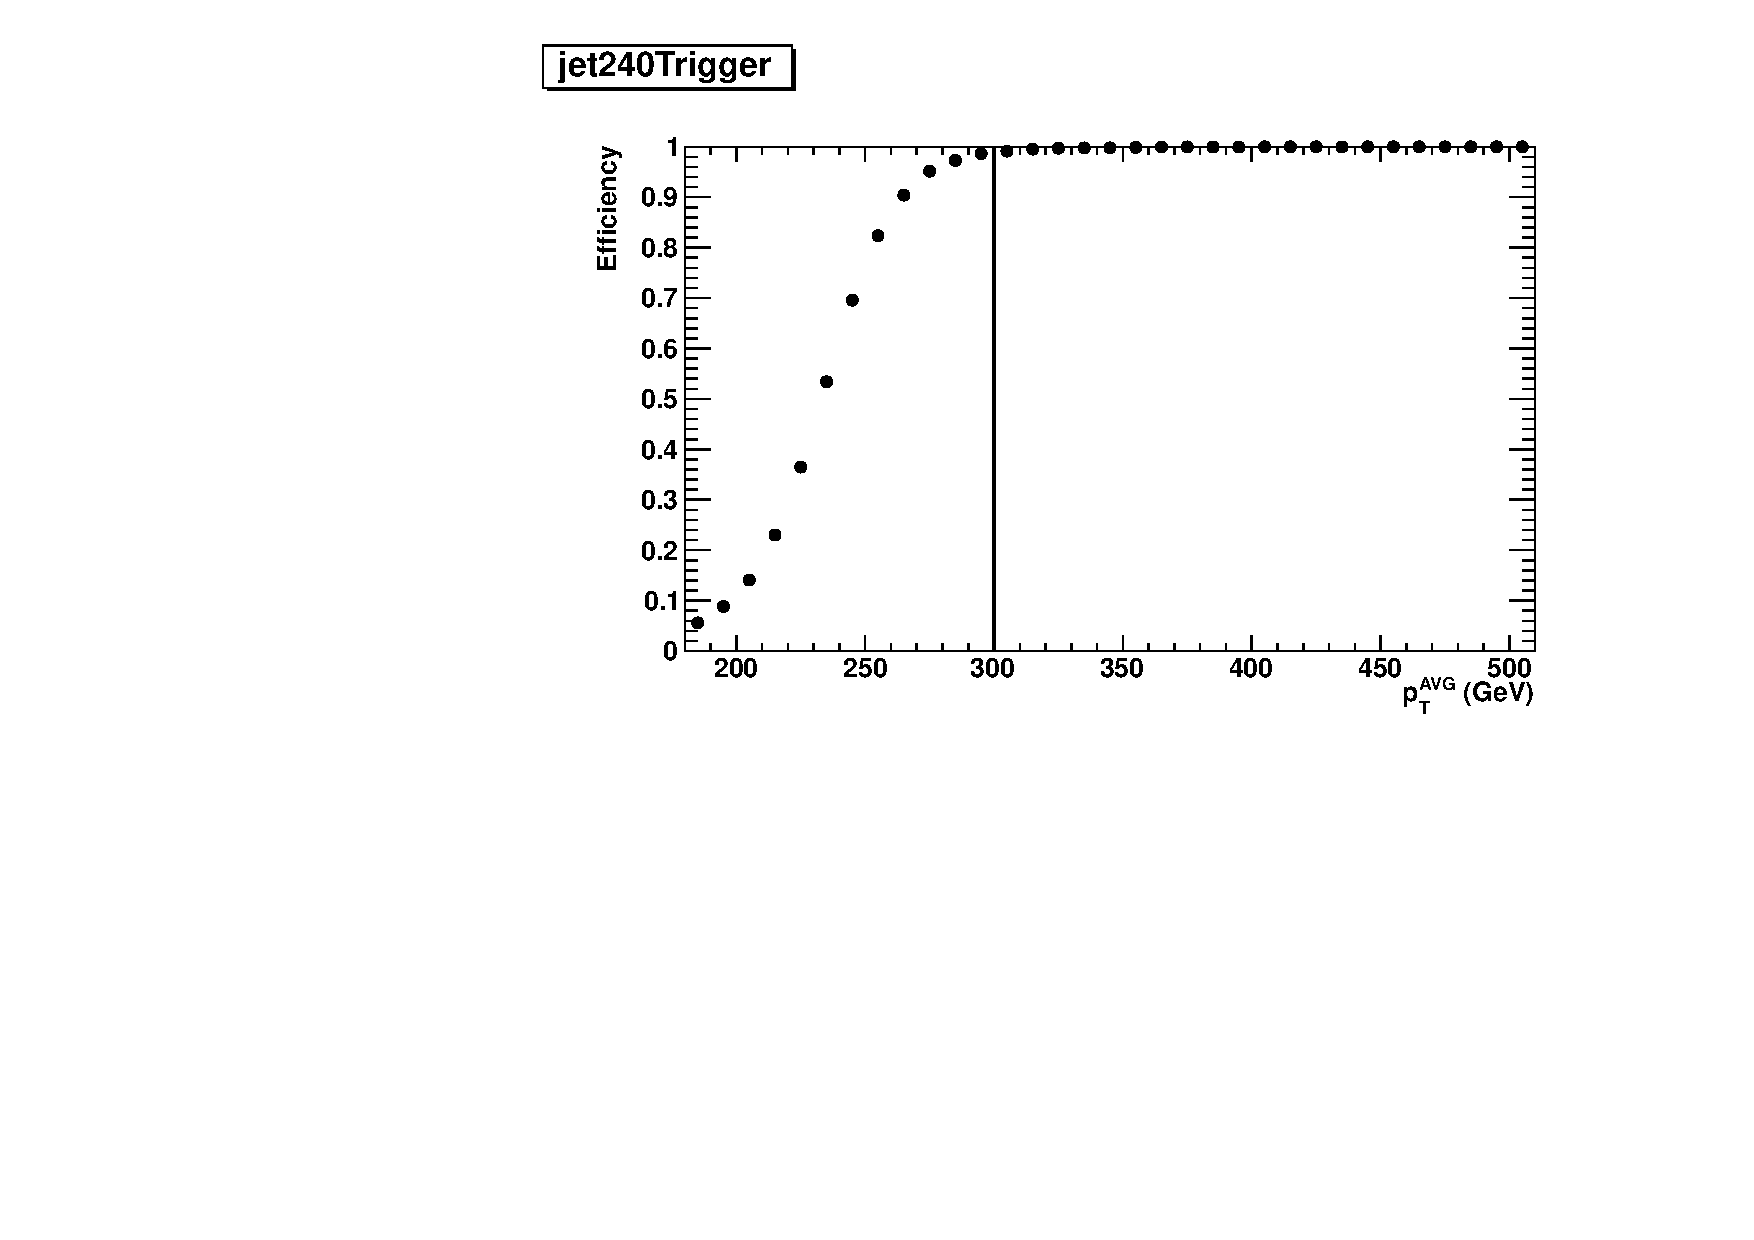
\includegraphics[width=0.6\textwidth]{figs/efficiency_jet240Trigger}}
\subfigure{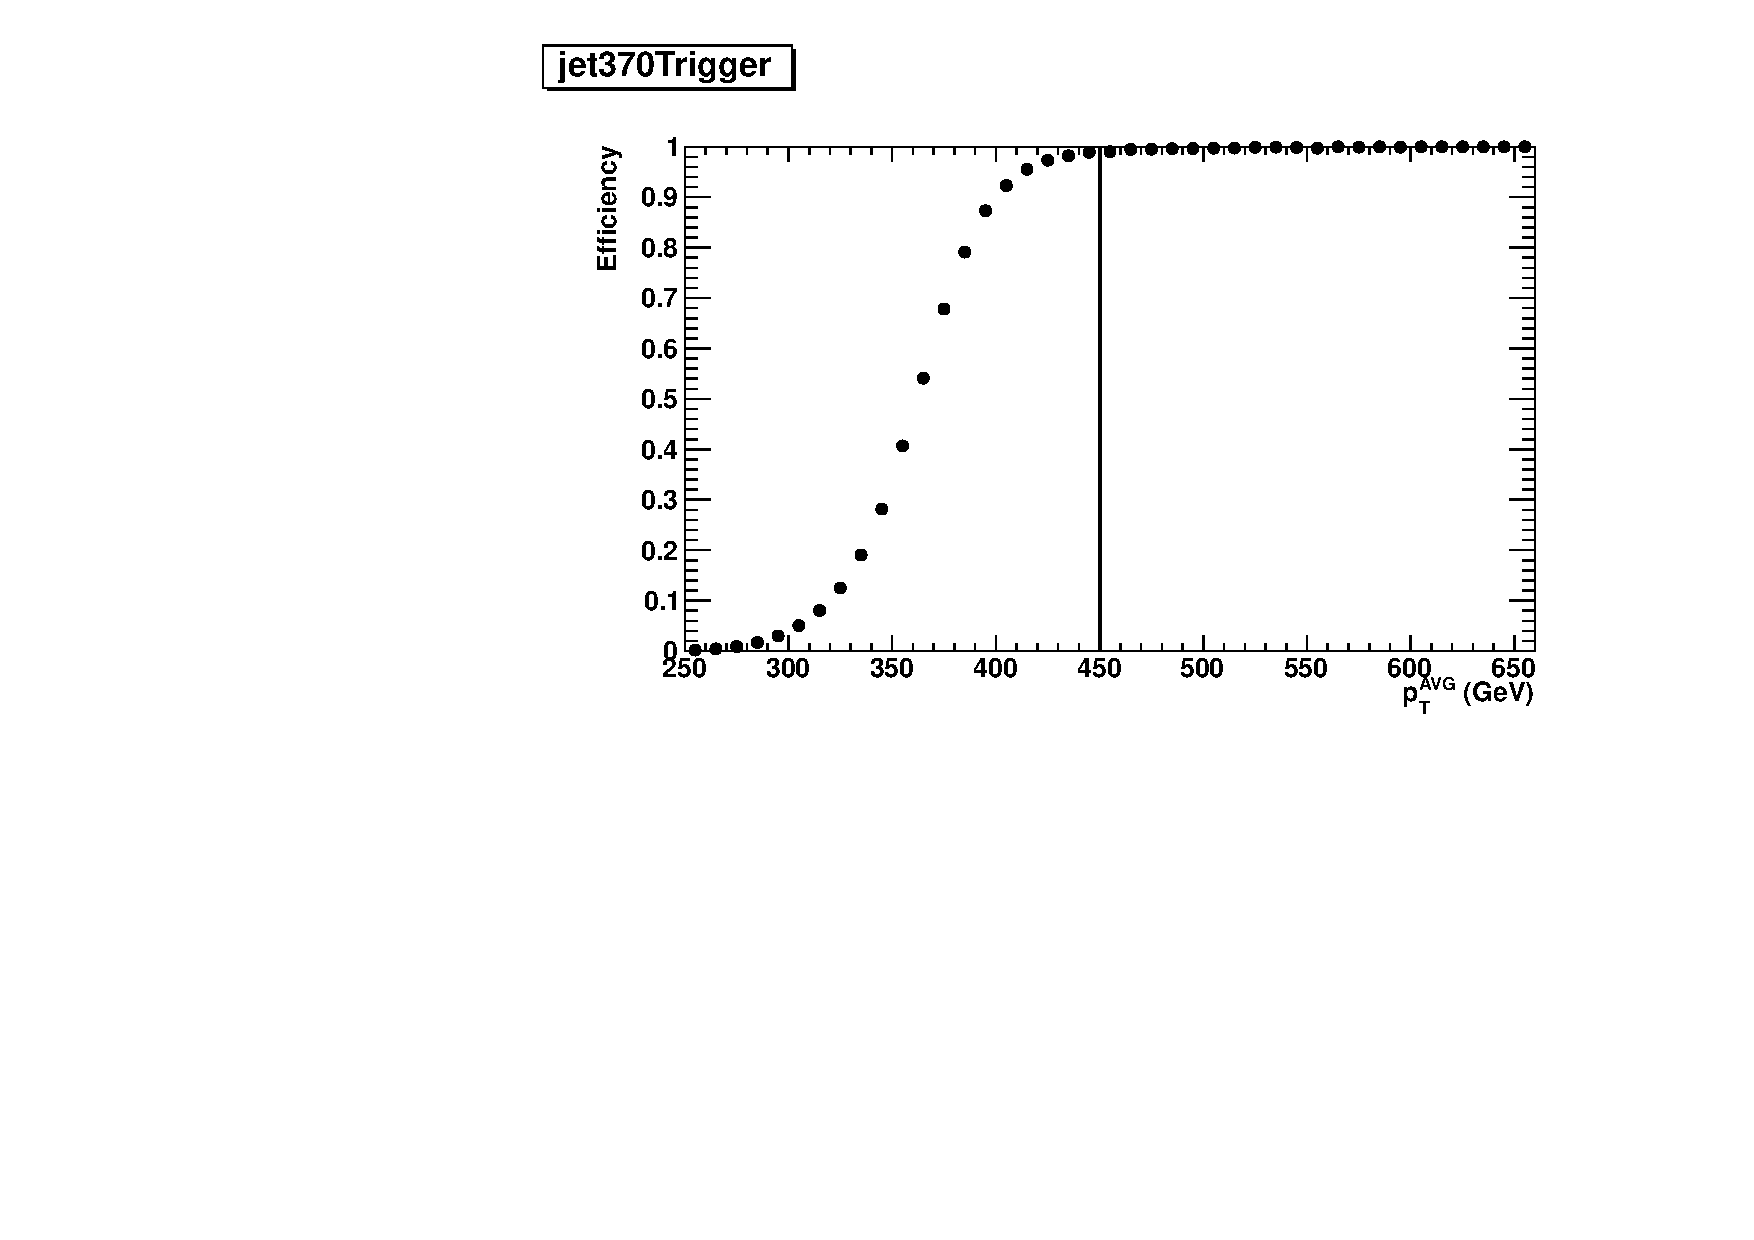
\includegraphics[width=0.6\textwidth]{figs/efficiency_jet370Trigger}}
\caption{Trigger efficiency as a function of $\pt^{AVG}$. 
\label{figs:efficiency_HLT}}
\end{figure}


\begin{table}[h]
  \centering
  \begin{tabular}{ |c|c|}
    \hline 
Jet60 & 0-150 \GeV   \\
Jet100& 150-220 \GeV \\
Jet190& 220-300 \GeV \\
Jet240& 300-450 \GeV \\
Jet370& $>$450 \GeV \\
   \hline 
  \end{tabular}
  \caption{Trigger efficiency turn-on values for all jet samples.\label{TriggerTurnOns}}
\end{table}



\subsection{Transverse momentum bin assignment}
\label{sec:ptBinAssignment}


The jet mass is correlated with the energy of the jet. As such,
it is necessary to measure the jet mass in bins of transverse 
momentum of the jet $\pt$. Since this analysis uses a dijet
sample, the average jet $\pt$ is used as a variable of interest ($\pt^{AVG}$).

The $\pt^{AVG}$ binning chosen is to be
as similar as possible to the V+Jets analysis in
Ref~\cite{cmsSMPJSVJ}.
It is also chosen such that only one dijet trigger contributes to each
bin in $\pt^{AVG}$. 
As such, the binning is shown in Table~\ref{tab:ptBins}.
In this case, to assure that the appropriate $\pt$ dependence
of the jet mass is captured for the various grooming algorithm,
the $\pt^{AVG}$ is evaluated for each of the grooming techniques. 


\begin{table}[h]
  \centering
  \begin{tabular}{ |c|c|}
    \hline 
    Bin & $\pt^{AVG}$ \\ 
    \hline
    %0 & 0-50 \GeVc \\
    1 & 50-125 \GeVc \\
    2 & 125-150 \GeVc \\
    3 & 150-220 \GeVc \\
    4 & 220-300 \GeVc \\
    5 & 300-450 \GeVc \\
    6 & 450-500 \GeVc \\
    7 & 500-600 \GeVc \\
    8 & 600-800 \GeVc \\
    9 & 800-1000 \GeVc \\
    10& 1000-1500 \GeVc \\
    11& $>$1500 \GeVc \\
    \hline 
  \end{tabular}
  \caption{Jet $\pt^{AVG}$ bins. \label{tab:ptBins}}
\end{table}
